\chapter{Hardware consideration}
\label{chap:hardware_consideration}
In this chapter we will see how to execute code fast and we will see that
hardware is an important factor on this.

Nowadays, optimization is rarely done on AST. So, our figure
\ref{fig:java_pipel}, even if we rework our AST to be optimized. A more
realistic pipeline in nowadays compiler is this one:
\begin{figure}[H]
     \centering
     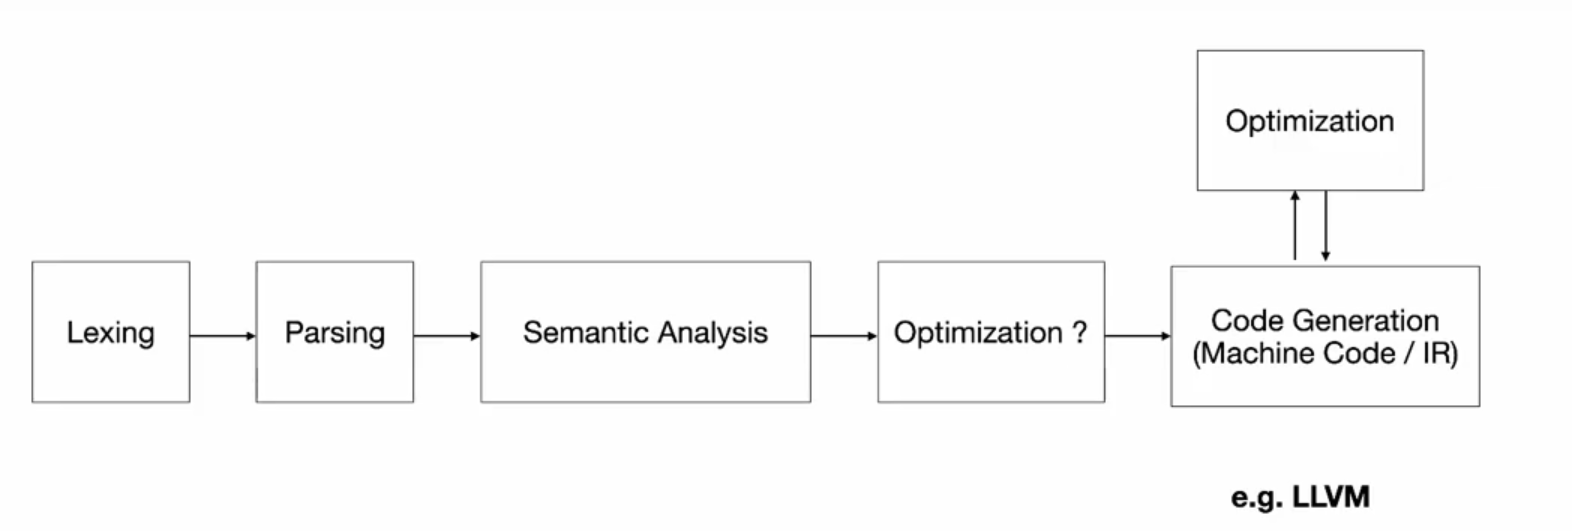
\includegraphics[scale=0.3]{realisticPipeline}
     \caption{LLVM pipeline}
     \label{fig:llvm_pipeline}
\end{figure}

Optimization is done on machine code(or close representation of it). It use
special data structure (graph) to optimize it. Other representation exists (see
slides). In cases of JIT, the optimization is run on the machine the program is
executed instead of the developer compiler.

We can also profile JIT with an interpreter that create a profile that will be
optimized.

\section{What makes program slow?}
The more instructions we have (exactly the number of CPU cycles) that are needed
to execute the program (i.e: 4Gz clock on a CPU means 4 billions of cycles per
second).

Memory access is also very slow (it is more a problem than CPU cycles). This is
often call the memory wall. An "everyday" concern with that problem for almost
every developer would be \textit{quick sort} vs \textit{merge sort}. Even if
both are in $\mathcal{O}(n log(n)$ (average case) with a worst case of
$\mathcal{O}(n^2)$ in quick sort. However, quick sort is faster than merge sort,
why? First of all, the worst case is rare, but also because quick sort has more
"memory locality" (jumps around in memory much less than merge sort).

\section{Memory hierarchy}
The following figure shows the memory hierarchy:
\begin{figure}[H]
     \centering
     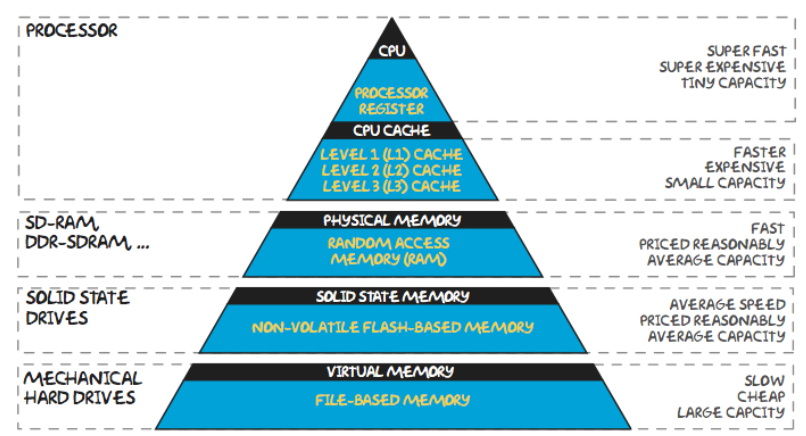
\includegraphics[scale=0.6]{MemoryHierarchy}
     \caption{Memory Hierarchy}
     \label{fig:mem_hierar}
\end{figure}
\theoremstyle{definition}
\begin{definition}[Register]
    Top of the hierarchy there are registers (very few of them, low capacity,
very expensive, they have to be managed explicitly).
\end{definition}
\theoremstyle{definition}
\begin{definition}[Caches]
    Just below register, they are managed automatically, the caches every access
    in the RAM.
\end{definition}
\theoremstyle{definition}
\begin{definition}[RAM]
    Main memory for the program, every time we use something it will be inserted
    in the cache.
\end{definition}

When we want to read something in the memory the CPU will first try to read in
L1 cache, if not found, L2, then L3. Let's say something is found in L3 it will
be re-write in L1 and L2 in order to speed-up future access, using the principle
of "if something is needed now, there is a high chance it will be needed again
very soon". 

Note that, concerning memory, the bigger it is, the slower it is but also, the
faster it is, the more extensive it becomes. Still, it is not the only issue, in
order to be fast, registers must be near the CPU, however, the CPU has a limited
amount of available space and the most of it is taken by instructions (and
gates). In the end, registers are not only a financial issue, but also a
performance one.

The last two layers, could be merge into one as "mechanical drives", here there
is a distinction between SSD and HDD. 

As many process are run in parallel, a process does not have direct access to
the memory, but to a virtual memory address space which will access the "real"
memory. If there is not enough space on the main memory (RAM) the virtual memory
address could be map to the the swap. Not that the memory of a program can only
exists either in RAM or in swap, but not in both at the same time. See speed
comparison on slide 8. Even RAM is 200 times slower than L1 will SSD is 3 000
000 times slower than L1.

Note that, "branch mispredict" is the estimation of time loose when we have to
branch (if statement). 

Of course, these times changes depending on the CPU and the technology
evolution.

Slide 9 shows the CPU cycle needed for different operation. As we can see,
memory write is one cycle. Indeed, we can gives the order to write, than do
other things. Still, there is a potential issue with that, if we need to read
from where we just wanted to write, we have to wait for it to write. Compilers
are sometimes able to optimize that but it is not always the case. We can also
see that floating point maths is slower than integer maths, mul/div slower than
add/sub, etc.

\section{Cache}
Each cache is composed of cache lines (slots). If we take a recent Intel Core i7
for example, it has a L1 cache of 32KB / 64B Lines, L2: 256KB / 64B Lines
(associativity: 8). What does it mean? Whenever RAM is accessed a 64B-aligned
chunk of memory is pulled into the caches (so, 64B-aligned just mean that we
load a multiple of 64 bytes in the cache). 

If we want to know the cache line index (in order to do cache lookup) the
formula is the following: $(address \% cache size) / 64$ (let's say address is
129, cache size is 32Kb truncating with 64 we get 1, which is the second line of
the cache).

Note that L1 does not contains the 32Kb most recently accessed memory because of
cache conflicts (address 1 and 129 would have the same cache line of 1). That's
where the associativity appears, an associativity of 8 means that up to 8
conflicts are allowed, there are 8 version of each cache line, in the end, it
means the the total memory has only a cache size of 4kb. Not that all "sub
caches" are checked in parallel.


Some other caches exists TLB (Translation lookaside buffer, maps the virtual
addresses to the real memory address) and instruction cache that contains the
CPU instructions.

\section{Instructions}
As we have seen before, instructions does not have the the same cost. As it is
CPU dependant, two CPUs can have different cost for the same instruction.

Details of CPU affect performance:
\begin{itemize}
    \item Memory caches
    \item Instruction pipelining
\end{itemize}

\subsection{Instruction pipelining}
Every instruction is executed in multiple stages: fetch(fetch the instruction),
decode(understanding the instruction structure and convert into to the real CPU
instruction (micro-code)), execute (execute the micro-code), writeback(write in
register if needed).

The idea is that, when we execute an instruction, we can decode the next one and
fetch the second one, doing that will allow to keep the pipeline as busy as
possible if it fails to do that it is called "pipeline stall". Note, that
sometimes, we are forced to have that stall, like in branch mispredict (in a if
statement, the CPU will try to predict the branch speculatively, if it is wrong,
it have to cancel the actual instruction and wait to fetch the next one. So, in
case of mispredict, we'll get some states that does nothing, waiting for the
"real" next instruction). An other way of pipeline stall is data dependency, it
occurs when an instruction depend on the result of an other instruction.
Compilers try to optimize (reorder instructions) that but it is not always
possible.


More advanced pipelining is Superscalar processors exploit ILP (Instruction
Level Parallelism) which runs multiple pipeline in simultaneously on the same
CPU core. It is used for independent instructions from the same program. These
pipelines must be filled explicitly with VLIW (Very Long Instruction Word).


Another variant is SMT (Simultaneous Multi-Threading), the most know is the
Intel's variant called "Hyper-Threading". It filled the pipeline with
instructions from another thread or process in order to be sure to keep the
pipeline busy. There is still a pitfall for that, as the two thread will access
the same cache (as running on the same core), it can be slower than running the
two threads separately because the second thread can pollute the cache for the
first thread and thus, degrade is performances.


There is also SIMD (Single Instruction Multiple Data) it is not really a
pipeline architecture but a capacity of processors to exploit data-level
parallelism. It use SIMD instruction that allow to run an instruction on an
array of data. It is very useful for image, sound processing, number crunching,
machine learning, etc. is SIMD always the solution? No! First it only on data on
which we want to use the same operation but also, data needs to be packed
together (contiguous in memory). Thus, even without SIMD it is already pretty
fast (as the would be cache in the same time) SIMD is just even faster.

\section{How can programmer improve performance?}
We should be very careful on algorithm and data structure that we use. We should
consider both average and worst case complexities, but also consider the
quantity and pattern of memory access. 

We should also give as much hints as possible to the compiler (as it is not
always possible for the compiler to infer it) some example could be the "final"
modifier of Java or storing an intermediate value instead of recomputing it.

Compilers are \textit{often} smart Truffle is sometimes used by final, even if
it's not supposed to. This is part of the compiler optimization budget.
Optimization is important but we don't want the compiler to loose all its time
doing that. Specify "final" allow it to not loosing time as it trust the developer.

In the end, compiler improve cache utilization (cache locality) but also improve
processor utilization (avoid pipeline stalls) and remove obstacles to optimization!